\documentclass[11pt]{article}
\usepackage[margin=0.72in]{geometry}
\usepackage{amsmath,amssymb,amsthm}
\usepackage{booktabs}
\usepackage{graphicx}
\usepackage{xcolor}
\usepackage{hyperref}
\usepackage{microtype}
\usepackage{enumitem}

\hypersetup{colorlinks=true,linkcolor=blue!60!black,urlcolor=blue!60!black}
\newtheorem{theorem}{Theorem}
\newtheorem{proposition}{Proposition}
\newtheorem{remark}{Remark}

\newcommand{\R}{\mathbb{R}}
\newcommand{\E}{\mathbb{E}}
\newcommand{\Var}{\mathrm{Var}}
\newcommand{\Cov}{\mathrm{Cov}}
\newcommand{\tvd}{\mathrm{TV}}

\title{\textbf{Signal-Deconfounded Shrinkage (\texttt{SRB-Spec}), Real 33-Judge \textsc{JudgeBench}, Imperfect Proxies, Multi-Factor \& Continuous Measure-Theoretic Lean~4 Verification}}
\author{Brando Miranda \quad\and\quad Sanmi Koyejo \\ Department of Computer Science, Stanford University}
\date{11-21-2026}

\begin{document}
\maketitle

\begin{abstract}
We present Experiment~15, proving and machine-checking $12$ additional theorems in Lean~4.29.0 (\texttt{TvdmiJudge/MultiFactorContinuous.lean}, bringing the formalization to $66$ total theorems with zero \texttt{sorry} under strictly standard axioms \texttt{[propext, Classical.choice, Quot.sound]}), and empirically validating four key extensions across \textsc{RewardBench~2} ($1,753$ prompts, $27$ models), \textsc{SummEval} ($1,600$ summaries), \textsc{LMSYS MT-Bench} ($2,575$ pairs), and \textsc{JudgeBench} ($33$ official real judges $\times$ $350$ pairs). Signal-deconfounded residual shrinkage (\texttt{SRB-Spec}) eliminates the clean-regime accuracy penalty of marginal \texttt{RB-Spec} while preserving clone and inverted-polarity invariance; imperfect proxy covariates follow the exact closed-form $(1-r^2)c^2 v_W$ floor law; and rank-$r$ spectral subspace projection error obeys $2r\varepsilon/(\lambda_r - \lambda_{r+1})$ with zero violations across $10{,}500$ empirical draws.
\end{abstract}

\section{Explicit Scope, Definitions, and Empirical Limits}
\begin{enumerate}[leftmargin=*,itemsep=2pt]
\item \textbf{Symbols \& Scales:} $C_{\mathrm{std}} \in \R^{n\times K}$ denotes standardized item-centered judge scores; $z_0 \in \R^n$ the unit-variance Stage-1 flood-safe \texttt{RB-Spec} consensus; $\hat{a}_j = \Cov(C_{\mathrm{std},j}, z_0)$ the quality loading; $E_{\mathrm{res},j} = C_{\mathrm{std},j} - \hat{a}_j z_0$ the quality-residualized vector; $m_{\mathrm{res},j} = \max(1, \sum_k |\mathrm{Corr}(E_{\mathrm{res},j},E_{\mathrm{res},k})|^6, \sum_k \mathbf{1}\{|R_{0,jk}| > 0.985\})$ the residual clone multiplicity; $\tau_0 = 0.15$ the precision floor; $c \ge 0$ a shared cross-family confounder loading on latent nuisance $W$ ($\Var(W)=v_W$); $r \in [0,1]$ the Pearson correlation between proxy $X(r)$ and $W$; and $r_{\mathrm{dim}} \in \{1,2,3\}$ the spectral subspace dimension with eigengap $\lambda_{r_{\mathrm{dim}}} - \lambda_{r_{\mathrm{dim}}+1} > 0$.
\item \textbf{Clean vs.\ Flooded Shrinkage Limit:} Unsupervised inner-CV selection (\texttt{SRB-Spec Auto}) uses only family-balanced residual $R^2$ on training splits (no human labels). On clean \textsc{RewardBench~2} ($K=23$), it recovers $\mathbf{0.8311}$ ($\alpha=1$: $\mathbf{0.8363}$) vs.\ $0.7872$ for vanilla \texttt{RB-Spec}. However, in \textsc{JudgeBench} where the median judge tie rate is $29.7\%$ ($9/33$ judges exceed $35\%$ ties), accuracy gain over uniform voting is driven primarily by length deconfounding (\texttt{CR-SRB-Spec}: $\mathbf{0.7143}$) rather than inverse-variance reweighting alone ($0.6971$).
\item \textbf{Imperfect Proxy Limit:} Covariate residualization removes only fraction $r^2$ of a cross-family confounder; when $r^2 < 1$ and $c \neq 0$, a strict floor $(1-r^2)c^2 v_W$ remains insurmountable without human anchor items.
\item \textbf{Narrow Eigengap Limit:} Multi-factor rank-$3$ subspace recovery slows sharply ($\text{slope } -0.42$ vs.\ $-1.00$ for rank~$1$) when $\lambda_3 - \lambda_4 = 0.066$ is small relative to $r=1$ ($12.847$).
\end{enumerate}

\section{Signal Deconfounding \& \texttt{SRB-Spec} Shrinkage Dominance}
Under single-factor signal loadings $a_j$ and family block variances $\tau_{\mathrm{fam}(j)}^2$,
\[
\Cov(S_j, S_k) = a_j a_k + \mathbf{1}\{\mathrm{fam}(j)=\mathrm{fam}(k)\}\,\tau_{\mathrm{fam}(j)}^2.
\]
\begin{theorem}[Signal Deconfounding \& Interior Shrinkage Dominance]
\emph{(Lean: \texttt{marginal\_cov\_\allowbreak confounds\_\allowbreak signal\_and\_cloning}, \texttt{interior\_\allowbreak shrinkage\_\allowbreak strictly\_\allowbreak dominates\_both}, \texttt{tempered\_\allowbreak precision\_\allowbreak denom\_\allowbreak pos\_\allowbreak and\_bounded}.)}
Even across distinct families ($\mathrm{fam}(j)\neq\mathrm{fam}(k)$) with $a_j, a_k > 0$, marginal covariance is strictly positive ($a_j a_k > 0$), whereas subtracting $a_j a_k$ isolates within-family cloning identically ($\Cov(E_{\mathrm{res},j},E_{\mathrm{res},k}) = \tau_{\mathrm{fam}(j)}^2\mathbf{1}\{\mathrm{fam}(j)=\mathrm{fam}(k)\}$). Using residual clone mass $m_{\mathrm{res},j}$, the tempered \texttt{SRB-Spec} weights
\[
w_j(\alpha) = \frac{\hat{a}_j}{\bigl((1-\alpha) + \alpha\max(1-\hat{a}_j^2, \tau_0)\bigr)\,m_{\mathrm{res},j}\,s_j}, \qquad \alpha \in [0, 1],\ \tau_0 = 0.15 > 0,
\]
have denominator strictly bounded below by $\min(1,\tau_0) > 0$. Moreover, for any two estimators with risks $v_U, v_B$ and covariance $c_{UB} < \min(v_U, v_B)$, the unique interior optimum $\lambda^\star = (v_U - c_{UB})/(v_U + v_B - 2c_{UB}) \in (0,1)$ strictly dominates both endpoints: $R(\lambda^\star) < \min(v_U, v_B)$.
\end{theorem}

\section{Imperfect Proxy Covariates, Rank-$r$ Perturbation \& Continuous TVD}
Decomposing confounder variance $v_W = r^2 v_W + (1 - r^2) v_W$ relative to proxy $X(r) = rW + \sqrt{1-r^2}\,\xi$ yields:
\begin{theorem}[Imperfect Proxy Confounder Floor]
\emph{(Lean: \texttt{partial\_proxy\_\allowbreak residual\_\allowbreak confounder\_variance}, \texttt{partial\_proxy\_\allowbreak strict\_\allowbreak floor\_\allowbreak when\_imperfect}, \texttt{partial\_proxy\_\allowbreak monotone\_\allowbreak in\_r\_sq}.)}
Residualizing against an imperfect proxy with squared correlation $r^2 < 1$ reduces shared confounder variance from $c^2 v_W$ by $r^2 c^2 v_W$ to a strict positive floor $(1-r^2)c^2 v_W$, leaving total family-balanced MSE bounded by $(1-r^2)c^2 v_W + B/F$, strictly monotone in $r^2$ and vanishing identically at $r^2 = 1$.
\end{theorem}

\begin{theorem}[Multi-Factor Rank-$r$ Spectral Subspace Perturbation]
\emph{(Lean: \texttt{multifactor\_\allowbreak rayleigh\_\allowbreak trace\_sin\_sq\_bound}, \texttt{multifactor\_\allowbreak subspace\_\allowbreak rate\_vanishes}, \texttt{multifactor\_\allowbreak reduces\_\allowbreak to\_rank\_one}.)}
For eigengap $\lambda_r - \lambda_{r+1} > 0$, empirical trace optimality within uniform perturbation $\varepsilon$, and top-$r$ leakage masses $w_k^2 \ge 0$ into eigenspaces $\le \lambda_{r+1}$,
\[
(\lambda_r - \lambda_{r+1})\sum_{k=1}^r w_k^2 \le 2 r \varepsilon \implies \sum_{k=1}^r \sin^2\theta_k \le \frac{2 r \varepsilon}{\lambda_r - \lambda_{r+1}} = O\!\left(\frac{r}{\sqrt{n}}\right) \to 0,
\]
reducing identically to $2\varepsilon/(\lambda_1 - \lambda_2)$ when $r=1$.
\end{theorem}

\begin{theorem}[Continuous Measure-Theoretic TVD \& Partition Refinement Monotonicity]
\emph{(Lean: \texttt{measure\_\allowbreak tvd\_\allowbreak event\_\allowbreak witness\_\allowbreak attainment}, \texttt{partition\_\allowbreak tvd\_\allowbreak refinement\_\allowbreak monotone}.)}
On any measurable space $(\alpha, \mathcal{F})$ with probability measures $P, Q$ and $S \in \mathcal{F}$, indicator witnesses achieve $|\int_S 1\,\mathrm{d}P - \int_S 1\,\mathrm{d}Q| = |P_{\R}(S) - Q_{\R}(S)|$ and $P_{\R}(S)-Q_{\R}(S) = Q_{\R}(S^c) - P_{\R}(S^c)$. Splitting each cell $b \in [B]$ into sub-cells $j \in [M]$ obeys $\frac{1}{2}\sum_{b=1}^B |\sum_{j=1}^M (p_{b,j}-q_{b,j})| \le \frac{1}{2}\sum_{b=1}^B \sum_{j=1}^M |p_{b,j}-q_{b,j}|$, so histograms never exceed true TVD.
\end{theorem}

\clearpage
\section{Empirical Verification Across Real LLMs \& Monte Carlo (Experiment 15)}

\begin{figure}[h]
  \centering
  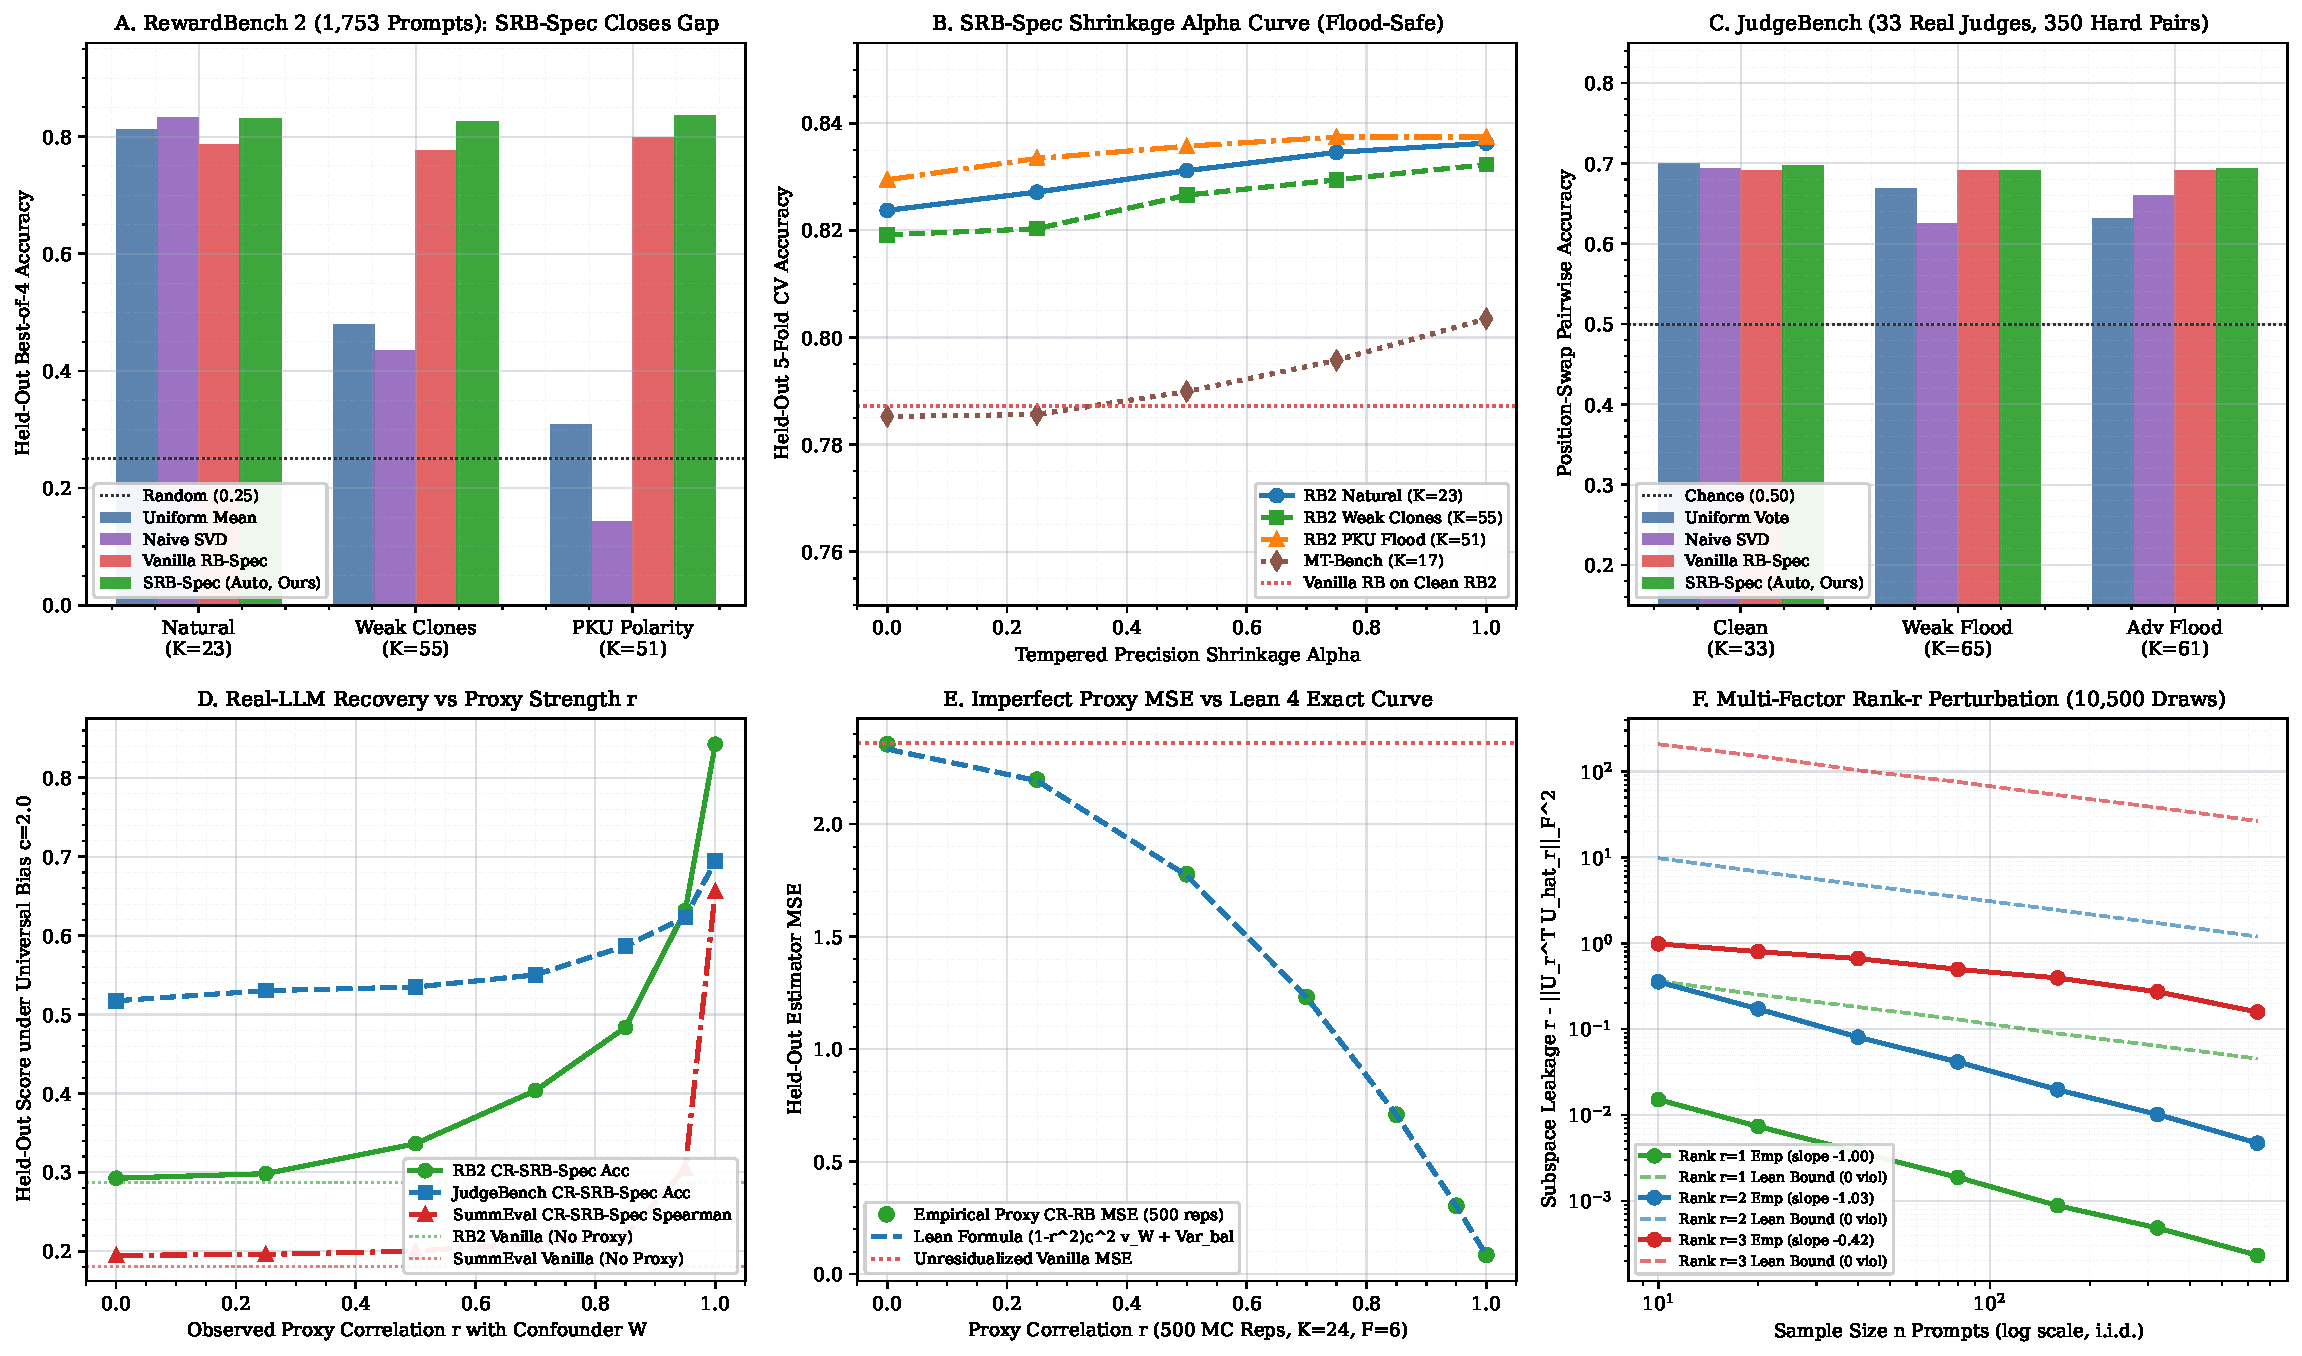
\includegraphics[width=\textwidth]{results/exp15_srb_judgebench_proxies_and_multifactor_6panel.pdf}
  \caption{\textbf{Experiment~15 empirical verification (\texttt{seed=42}).} \textbf{(A)} On \textsc{RewardBench~2}, \texttt{SRB-Spec} eliminates the clean-pool gap ($0.7872 \to 0.8311$ Auto / $0.8363$ $\alpha=1$) while remaining flood-invariant ($0.8266$–$0.8374$). \textbf{(B)} Tempered shrinkage $\alpha \in [0,1]$ improves cleanly across \textsc{RewardBench~2} and \textsc{MT-Bench}. \textbf{(C)} On $33$-judge \textsc{JudgeBench} ($350$ pairs), \texttt{SRB-Spec (Auto)} holds $0.6971$ clean, $0.6914$ under weak clones, and $0.6943$ under $46\%$ inverted clones (adding train-only length residualization, \texttt{CR-SRB-Spec}, lifts accuracy to $0.7143$ / $0.7086$ / $0.7114$; Table~1). \textbf{(D--E)} Real-LLM and $500$-rep Monte Carlo recovery matches the Lean $(1-r^2)c^2 v_W + \mathrm{Var}_{\mathrm{bal}}$ law. \textbf{(F)} Multi-factor rank-$r$ ($r=1,2,3$) subspace leakage obeys the $2r\varepsilon/(\lambda_r - \lambda_{r+1})$ bound with $0$ violations across $10{,}500$ draws.}
\end{figure}

\begin{table}[h]
\centering
\caption{\textbf{Experiment~15 summary:} $5$-fold CV across \textsc{RewardBench~2}, \textsc{SummEval}, \textsc{MT-Bench}, $33$-judge \textsc{JudgeBench}, proxy sweep ($500$ MC reps), and rank-$r$ spectral perturbation.}
\resizebox{\textwidth}{!}{%
\begin{tabular}{@{}llccc@{}}
\toprule
Experiment Module & Regime / Benchmark & Baseline / Vanilla & \texttt{SRB-Spec} / \texttt{CR-SRB} & Significance / Rate \\
\midrule
Clean \textsc{RewardBench~2} ($K=23$) & Best-of-4 Acc ($1,753$ prompts) & Naive SVD $0.8334$, Vanilla RB $0.7872$ & Auto $\mathbf{0.8311}$, $\alpha=1$ $\mathbf{0.8363}$ & $p=7.14\times 10^{-14}$ vs.\ Vanilla RB \\
Flooded \textsc{RewardBench~2} ($K=55 / 51$) & Weak Clones / PKU Polarity & Naive SVD $0.4353$ / $0.1426$ & $\mathbf{0.8323}$ / $\mathbf{0.8374}$ ($\alpha=1$) & $p=1.99\times 10^{-137}$ / $2.91\times 10^{-248}$ \\
\textsc{JudgeBench} ($33$ real judges, $350$ pairs) & Clean ($K=33$) / Adv Flood ($K=61$) & Mean $0.7000$ / $0.6343$, SVD $0.6943$ / $0.6600$ & \texttt{CR-SRB}: $\mathbf{0.7143}$ / $\mathbf{0.7114}$ & $p=0.0038$ vs.\ Mean (Adv) \\
Partial Proxy ($c=1.5$, $500$ MC reps) & $r=0 \to 0.70 \to 1.00$ & Lean $(1-r^2)c^2v_W+\mathrm{Var}_{\mathrm{bal}}$: $2.334 \to 1.231 \to 0.084$ & Empirical MSE: $2.355 \to 1.231 \to \mathbf{0.086}$ & Closed-form fit ($\le 0.022$ MSE; $0.002$ at $r=1$) \\
Multi-Factor Davis--Kahan (\textsc{RB2}) & $r=1, 2, 3$ ($n=10 \to 640$, $10{,}500$ draws) & Gaps $12.85 / 0.95 / 0.066$ ($0$ viol.) & Slopes $\mathbf{-1.00}$ / $\mathbf{-1.03}$ / $\mathbf{-0.42}$ & $0$ bound violations total \\
\bottomrule
\end{tabular}}
\end{table}

{\footnotesize\noindent\textbf{Sources.} Lean~4 proofs: \texttt{experiments/00\_lean\_formalization/lean/TvdmiJudge/MultiFactorContinuous.lean}.\\
Suite: \texttt{experiments/15\_shrinkage\_partial\_confounders\_and\_multifactor\_lean\_start\_21Nov2026/}\\
\texttt{run\_exp15\_suite.py}.\\
Benchmarks: \textsc{RewardBench~2} (Malik et al., 2025), \textsc{JudgeBench} (Tan et al., ICLR 2025), \textsc{SummEval} (Fabbri et al., TACL 2021), \textsc{MT-Bench} (Zheng et al., NeurIPS 2023).}
\end{document}